\iflong

\section{\gls{cat} Project}
Parekh et al. \cite{delphi} began the \gls{cat} Project development by identifying the core concepts of cybersecurity using a Delphi process. A Delphi process is a rigorous and structured method for creating consensus among experts about potentially contentious issues, such as what subset of concepts should be included on the \gls{cci} \cite{original_delphi}. This process identified five concepts to include in the \gls{cci} seen in Table \ref{tab:topics} \cite{delphi}. From these concepts, Sherman et al. \cite{scenarios} developed cybersecurity scenarios that require students to understand these concepts. For example, a scenario that covers concept \gls{c} involves a hypothetical government facility where the defenses and biometric authentication methods are defined. This scenario allows for questions on potential attacks that exploit this scenario.

Using these scenarios, Scheponik et al. \cite{misconceptions} performed think-aloud interviews to discover students' misconceptions and problematic reasoning \cite{jcerp}. Example forms of problematic reasoning include students' beliefs that encryption protects against most any cybersecurity threat or the belief that cybersecurity threats come only from outside an organization.

Using what was learned from these interviews, \gls{cci} items were created using the same scenarios. Each \gls{cci} item consists of a scenario, a stem (i.e., a question about the scenario), and five multiple-choice options. The wrong answers (distractors) were created based on the interview findings.

\fi

\section{Validity}

Validity is the set of arguments and evidence that establish whether and how an assessment tool can be used to measure students' knowledge \cite{douglas_purzer}. When designing an assessment tool, the National Research Council recommends establishing a cognitive framework for the assessment tool \cite{knowing_what_students_know}. This cognitive framework defines what knowledge in a topic should be assessed and the ways in which students reveal their knowledge, or lack of knowledge, about that topic. Prior work on the \gls{cat} Project has focused on establishing this cognitive framework, providing baseline arguments for the validity of the \gls{cci}.



\section{Classical Test Theory (CTT)}


\gls{ctt} is often the first scoring paradigm used to evaluate an instrument because it can be used with smaller sample sizes \cite{og_ctt}. With 142 students in the pilot, \gls{ctt} is more practical than more exhaustive analytics like \gls{irt}. Despite not being as powerful as \gls{irt}, \gls{ctt} allows us to find problematic questions and distractors and suggest modifications with a smaller number of students. This analysis enables more rapid iteration and improvement of the \gls{cilabel}.

\section{Reliability}


Reliability is a measure of the likelihood that repeated measurements of the same student will yield the same score. If an assessment tool is not reliable, it cannot be valid.

In \gls{ctt}, the core assumption is that a students' \textit{observed score (X)} consists of two hypothetical values: a students' \textit{true score (T)} and some random \textit{error (E)} \cite{og_ctt}. The students true score would be the score of an infinite number of independent administrations of the test \cite{true_score}.  This model is expressed symbolically as (X = T + E) \cite{dlci}. A reliable instrument minimizes the error so the observed score best reflects the students' understanding. 

The conventional measurement used for internal reliability is Cronbach's $\alpha$.  Cronbach's $\alpha$ is ``an estimate of the correlation between two random samples of items from a universe of items like those in the test" \cite{og_cronbach}. We can determine Cronbach's $\alpha$  without taking the instrument multiple times if two conditions are met. The conditions are (1) the instrument measures a single trait (2) the item is either correct or incorrect \cite{dlci}. A reliable instrument will lead to $\alpha$ values that are close to 1.  There is no universally acceptable Cronbach value, but 0.8 is considered good and 0.7 is the minimum value considered satisfactory according to Panayiotis \cite{panayiotis} and Jorion et al. \cite{jorian}.

Cronbach's $\alpha$ can also be used to coarsely evaluate the quality of each item. The addition of each item should increase the overall reliability of the instrument\cite{dlci}. By removing an item and then recalculating the $\alpha$ value, we can judge the quality of that specific item. When the removal of an item increases the value of $\alpha$, it is particularly poor and should be removed.


The standard error is a function of $\alpha$ and defines a confidence interval for each student's true score. Standard error is calculated using ($SE = S_x \sqrt{1-\alpha}$) where $S_X$ is the standard deviation of the sample and $\alpha$ is the Cronbach's $\alpha$. When the standard error is small, we can be confident students with different observed scores have different true scores. 


\section{Difficulty and Discrimination}

Reliability alone does not indicate the instrument provides a valid representation of students' knowledge. The validity of the instrument can be further established looking at each item's difficulty and discrimination. The difficulty of an item is the fraction of students with the correct response \cite{og_ctt}.  Each item of the instrument should have a difficulty in the range of 0.2 to 0.8 \cite{dlci, jorian}. When the difficulty is outside this range, it does not effectively separate students of a different understanding. To effectively separate students having a balance of difficulty within the acceptable range is ideal.

The discrimination of an item is the point-biserial correlation between the item and the overall performance \cite{jorian}. An item with low discrimination has weaker students (low total scores) perform similarly to stronger students (high total scores) on that item. A good item will have a discrimination of at least 0.2 \cite{dlci}. \iflong An item with proper discrimination and difficulty will fall within the largest square area as noted by the dotted lines in Figure \ref{fig:ideal}.\fi 

\iflong
\begin{figure}[ht]
    \begin{center}
    \advance\leftskip-3cm
    \advance\rightskip-3cm
    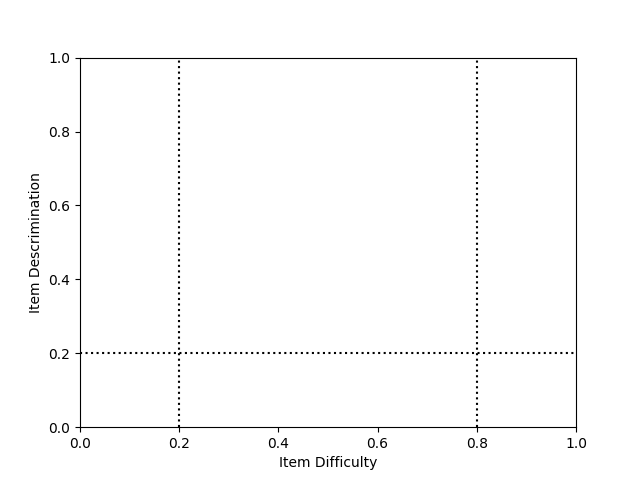
\includegraphics[scale=.5]{images/graph.png}
    \caption{Validity of Discrimination and Difficulty}
    \label{fig:ideal}
\end{center}
\end{figure}
\fi

\iflong
\section{Distractor Analysis}
\fi
\ifshort
\section{Topic Agreement and Distractor Analysis}
\fi


Distractor analysis can be used to analyze an item that's inclusion doesn't improve $\alpha$ or has a difficulty and discrimination outside the accepted range. To analyze distractors we split the students into tertiles (thirds) according to total scores. After splitting the students, take the proportion of test takers selecting each response \cite{og_ctt}. There are certain trends we expect to see. (1) The percentage of students selecting the correct answer should increase from the bottom third to the top third. (2) The item's difficulty for the top third of students should be near the upper range of accepted difficulty. (3) Each distractor is expected to have a negative discrimination value \cite{distractor}. A distractor's discrimination value is calculated by setting it as the correct answer and re-grading the student's responses. A distractor with a negative discrimination is selected more by weaker students. %If these trends do not appear the distractor may be the issue.

\section{Concept Subgroups}

Cronbach's $\alpha$ can be applied to a group of items called a \textit{subgroup}. In our case, the subgroup consists of the 5 items designed to cover the same concept. These subgroups can be evaluated separately to assess reliability to determine whether these subgroups can be tested individually. Ideally, the concept should have a reliability similar to the overall instrument. In practice, having a similar reliability to the entire instrument is difficult because each subgroup has fewer items. 


\iflong

\section{Previous Work}
\subsection{Concept Inventory Evaluation}

Because a test cannot be universally valid for every population or use, we need to carefully define the contexts, populations, and uses for which the \gls{cci} is valid. The \gls{cci} is intended to measure the cybersecurity conceptual knowledge of students who have completed a first course in cybersecurity. Cybersecurity is taught to an increasingly wide range of stakeholders, such as policy makers, computer scientists, medical professionals, and business professionals whose courses vary in focus and depth. Because of this high variance, we have chosen to optimize the \gls{cci} for the largest population of cybersecurity professionals - computer scientists. While the \gls{cci} may provide useful insights about the conceptual knowledge of policy makers or others, our goal is to have the tool provide the most insight about computer science students. 

Once an assessment tool is created, it should be administered to its targeted demographic and be statistically evaluated. \glspl{cilabel} can be powerful instruments if they actually measure students' conceptual knowledge. A minority of \glspl{cilabel} have been scrutinized using measurement or test development theories to justify being a valid and reliable research instrument \cite{dlci}. Jorian et al. \cite{jorian} outline three basic criteria of a valid \gls{cilabel}: \gls{cilabel} indicates overall understanding of the concepts, \gls{cilabel} indicates understanding of a specific concept, \gls{cilabel} indicates misconceptions or student errors.

 Jorion et al. recommend using a series of statistical tests to demonstrate whether a \gls{cilabel} meets these criteria. They recommend beginning analysis of \gls{cilabel} using \gls{ctt}. \gls{ctt} argues that an assessment tool should minimize error, possess items that all test a single construct, possess items that are neither too hard or too easy, and possess items that each provide a good estimate of a students' overall ability. 

\fi